\documentclass[11pt,a4paper]{article}

\usepackage[utf8]{inputenc}
\usepackage[T1]{fontenc}
\usepackage{lmodern}
\usepackage[margin=2.5cm]{geometry}
\usepackage{amsmath,amssymb,amsthm}
\usepackage{booktabs}
\usepackage{graphicx}
\usepackage{xcolor}
\usepackage{enumitem}
\usepackage[hidelinks]{hyperref}

% ---------------------------------------------------------------------------
% Notation macros (keep in sync with Section 1)
% ---------------------------------------------------------------------------
\newcommand{\D}{\mathcal{D}}          % set of duties
\newcommand{\A}{\mathcal{A}}          % arcs of the compatibility graph
\newcommand{\K}{\mathcal{K}}          % employee pool
\newcommand{\Wft}{W}                  % FT max working time
\newcommand{\Tft}{T}                  % FT max total time (spread)
\newcommand{\TODO}[1]{\textcolor{red}{\textbf{TODO:} #1}}

\newtheorem{proposition}{Proposition}
\theoremstyle{remark}
\newtheorem*{remark}{Remark}

\title{Model-driven Decision Methods\\[0.3em]
       \large Project n.~2 --- Transport Crew Duty Covering}
\author{}
\date{\today}

\begin{document}

% ===========================================================================
% Title page (mandatory content: group number, members, project number,
% verbatim assignment)
% ===========================================================================
\begin{titlepage}
  \centering
  {\Large Università di Pisa\par}
  \vspace{0.5em}
  {\large Model-driven Decision Methods --- A.Y.~2026/2027\par}
  \vspace{3em}
  {\LARGE\bfseries Project n.~2\par}
  \vspace{0.5em}
  {\Large Transport Crew Duty Covering\par}
  \vspace{3em}

  {\large \textbf{Group 1}\par}
  \vspace{1em}
  \begin{tabular}{lll}
    \toprule
    \textbf{Name Surname} & \textbf{Matricola} & \textbf{E-mail} \\
    \midrule
    Iachim Cristian & 744069 & c.iachim@studenti.unipi.it \\
    \bottomrule
  \end{tabular}

  \vspace{3em}
  \begin{flushleft}
  \textbf{Project assignment (verbatim):}
  \end{flushleft}
  \begin{quote}
  \small
  A transport company has to cover a set of driving duties with the available
  personnel. Each employee can perform different subsets of the duties; the
  subsets are implicitly specified under the form of a (given) ``compatibility
  graph''. That is, for each duty its starting time and the ending time are
  given; furthermore, for any pair of duties it is known the time that it takes
  to move from the place where the first one ends to the place where the other
  one starts, so that it is known whether or not it is possible for the same
  employee to perform both in sequence. Union regulations set for each employee
  a maximum working time (sum of the driving time) and a maximum total time
  (difference between the start of his first duty and the end of its last one).
  Employees can be both half-time or full-time; the former have maximum working
  time and total time half than the latter, but cost 60\% as much. The problem
  is to assign a feasible set of duties to an appropriate number of employees
  (of which there is an unlimited supply, of either type) in order to have each
  duty performed by exactly one employee, at minimum total cost.
  \end{quote}

  \vfill
  {\small Report version: Phase 2 draft (Sections 1--4) --- \today\par}
\end{titlepage}

\tableofcontents
\newpage

% ===========================================================================
\section{Problem description and mathematical models}
\label{sec:model}
% Milestone 1
% ===========================================================================

% ===========================================================================
% Section 1 -- Problem description and mathematical models
% ===========================================================================

\subsection{Notation}
\label{sec:notation}

\paragraph{Duties.}
Let $\D=\{1,\dots,n\}$ be the set of driving duties. Duty $i$ starts at time
$s_i$ and ends at time $e_i>s_i$; its driving time is $d_i=e_i-s_i$. For every
ordered pair $(i,j)$ of distinct duties, $t_{ij}\ge 0$ is the time needed to
move from the place where $i$ ends to the place where $j$ starts. All times are
integers (minutes) in the horizon $[0,H]$, with $H=\max_i e_i$.

\paragraph{Compatibility graph.}
Duty $j$ can be performed after duty $i$ by the same employee if and only if
the employee reaches the start of $j$ in time:
\begin{equation}\label{eq:arc}
  (i,j)\in\A \iff e_i+t_{ij}\le s_j .
\end{equation}
$G=(\D,\A)$ is the (given) compatibility graph. Since $(i,j)\in\A$ implies
$s_i<e_i\le s_j$, sorting duties by start time gives a topological order, so
$G$ is a \emph{directed acyclic graph} (DAG).

\paragraph{Employee types.}
There are two types $\tau\in\{\mathrm{F},\mathrm{H}\}$ (full-time,
half-time), each in unlimited supply, with
\[
  (W_{\mathrm F},T_{\mathrm F},c_{\mathrm F})=(W,\;T,\;1),\qquad
  (W_{\mathrm H},T_{\mathrm H},c_{\mathrm H})=(W/2,\;T/2,\;0.6),
\]
where $W_\tau$ is the maximum working time, $T_\tau$ the maximum total time
and $c_\tau$ the cost of one employee of type $\tau$ (normalised so that a
full-time employee costs $1$).

\paragraph{Shifts.}
A \emph{shift} is the ordered sequence of duties $p=(i_1,\dots,i_m)$
performed by one employee. It is \emph{feasible for type $\tau$} if
\begin{enumerate}[label=(S\arabic*)]
  \item $p$ is a path in $G$: $(i_\ell,i_{\ell+1})\in\A$ for
        $\ell=1,\dots,m-1$;
  \item working time: $\sum_{\ell=1}^m d_{i_\ell}\le W_\tau$;
  \item total time (``spread''): $e_{i_m}-s_{i_1}\le T_\tau$.
\end{enumerate}
We write $\Omega_\tau$ for the set of feasible shifts of type $\tau$. The
problem is to partition $\D$ into shifts, give each shift a type for which it
is feasible, and minimise the total cost $\sum c_\tau$ over the shifts used.

\subsection{Assumptions and interpretation choices}
\label{sec:assumptions}

The assignment leaves some details open. We fix them as follows (items marked
($\ast$) are ones we would like the lecturer to confirm).

\begin{enumerate}[label=(A\arabic*)]
  \item\label{ass:work} ($\ast$) \emph{Working time counts only the driving
    of the duties}, $\sum_{i\in p}d_i$. Deadhead movements $t_{ij}$ between
    duties are not counted, although they do count in the total time, since
    they lie between the start of the first duty and the end of the last.
    If deadheads must count too, formulation~(AF) below handles it by adding
    $t_{ij}$ to the arc weights in~\eqref{af:work}.
  \item\label{ass:cost} \emph{Cost is a fixed amount per employee used}
    ($1$ or $0.6$), independent of how many hours they actually work.
  \item\label{ass:wt} \emph{$W<T$.} Working time never exceeds total time
    (duties do not overlap), so if $W\ge T$ the working-time limit is redundant.
    The interesting case is $W<T$, and all our instances satisfy it.
  \item\label{ass:single} \emph{Every duty can be covered alone by a full-time
    employee}, i.e.\ $d_i\le W$ for all $i$; otherwise the instance is
    infeasible. Duties with $d_i>W/2$ can only be covered by full-time
    employees.
  \item\label{ass:tri} \emph{Triangle inequality (only where stated).}
    Formulation~(AF) works for an arbitrary DAG $G$, as the assignment speaks
    of a ``given'' graph. Formulation~(CF) additionally needs $G$ to be
    transitive. This is guaranteed when
    $t_{ij}\le t_{ik}+t_{kj}$, which holds whenever transfer times are
    shortest-path or Euclidean travel times between locations
    (Proposition~\ref{prop:transitive}).
\end{enumerate}

\begin{proposition}\label{prop:transitive}
If the transfer times satisfy $t_{ik}\le t_{ij}+t_{jk}$ for all $i,j,k$, then
$G$ is transitive.
\end{proposition}
\begin{proof}
Let $(i,j),(j,k)\in\A$. Then
$e_i+t_{ik}\le e_i+t_{ij}+t_{jk}\le s_j+t_{jk}\le e_j+t_{jk}\le s_k$,
hence $(i,k)\in\A$.
\end{proof}

\begin{remark}
Every half-time shift is also a feasible full-time shift
($\Omega_{\mathrm H}\subseteq\Omega_{\mathrm F}$), so a shift in
$\Omega_{\mathrm H}$ is always given to the cheaper half-time employee. Per
unit of working time, full-time employees are cheaper ($1/W$ against
$1.2/W$). Half-time employees pay off only for ``short'' shifts, those with
working time at most $W/2$ and spread at most $T/2$, that a full-time employee
would leave largely idle. This trade-off is what makes the mix of types
non-trivial.
\end{remark}

\subsection{Compact formulations}
\label{sec:compact}

Both compact models use an explicit pool of candidate employees
$\K=\K_{\mathrm F}\cup\K_{\mathrm H}$, with $|\K_\tau|=U_\tau$. Employee
$k\in\K_\tau$ has $(W_k,T_k,c_k)=(W_\tau,T_\tau,c_\tau)$. The pool must be
large enough not to cut off every optimal solution. $U_{\mathrm F}=n$ is
always valid, and so is $U_{\mathrm H}=|\{i:d_i\le W/2\}|$. Given the cost
$\bar z$ of any feasible solution (e.g.\ from a greedy heuristic), an optimal
solution uses at most $\lfloor\bar z\rfloor$ full-time and
$\lfloor\bar z/0.6\rfloor$ half-time employees, which gives much smaller
pools.

\subsubsection{Arc-flow formulation (AF)}

Add a source $\sigma$ and a sink $\omega$ to $G$:
$\bar\A=\A\cup\{(\sigma,i):i\in\D\}\cup\{(i,\omega):i\in\D\}$. For a node
$v$, $\delta^-(v)$ and $\delta^+(v)$ are its entering and leaving arcs in
$\bar\A$. The binary variable $z^k_a$ equals $1$ if employee $k$ uses
arc $a\in\bar\A$. Arc $(\sigma,i)$ means ``$i$ is the first duty of $k$'',
arc $(i,\omega)$ means ``$i$ is the last one''.
\begin{align}
\text{(AF)}\quad
\min\;& \sum_{k\in\K} c_k \sum_{i\in\D} z^k_{\sigma i} \label{af:obj}\\
\text{s.t.}\;
& \sum_{k\in\K}\sum_{a\in\delta^-(i)} z^k_a = 1
      && i\in\D \label{af:cover}\\
& \sum_{a\in\delta^-(i)} z^k_a-\sum_{a\in\delta^+(i)} z^k_a = 0
      && i\in\D,\;k\in\K \label{af:flow}\\
& \sum_{i\in\D} z^k_{\sigma i}\le 1
      && k\in\K \label{af:one}\\
& \sum_{i\in\D} d_i\!\sum_{a\in\delta^-(i)} z^k_a \le
      W_k\sum_{i\in\D} z^k_{\sigma i}
      && k\in\K \label{af:work}\\
& \sum_{i\in\D} e_i\, z^k_{i\omega}-\sum_{i\in\D} s_i\, z^k_{\sigma i}
      \le T_k\sum_{i\in\D} z^k_{\sigma i}
      && k\in\K \label{af:spread}\\
& z^k_a\in\{0,1\} && a\in\bar\A,\;k\in\K. \nonumber
\end{align}
Constraint~\eqref{af:cover} covers each duty exactly once,
\eqref{af:flow}--\eqref{af:one} make each employee follow at most one
$\sigma$--$\omega$ path, and \eqref{af:work}--\eqref{af:spread} enforce the
union rules. Because $k$ has exactly one first and one last duty when active,
the spread can be written \emph{without big-$M$ constants}: the two sums
in~\eqref{af:spread} pick out $e_{\text{last}}$ and $s_{\text{first}}$.
Multiplying the right-hand sides by the activation
$y_k:=\sum_i z^k_{\sigma i}$ adds nothing for integer solutions (an inactive
employee has zero left-hand side) but tightens the LP relaxation.

\begin{proposition}\label{prop:af}
For any DAG $G$, the integer solutions of (AF) correspond exactly to the
partitions of $\D$ into feasible shifts with a type assigned to each, and the
objective~\eqref{af:obj} equals the cost of the partition.
\end{proposition}
\begin{proof}
Fix $k$ with $y_k=1$. By~\eqref{af:cover}, every duty has in-flow at most $1$
under $k$. By~\eqref{af:flow} and~\eqref{af:one}, the arcs used by $k$ form a
flow of value $1$ from $\sigma$ to $\omega$. Since $G$ is acyclic, this flow
contains no cycle and is a single $\sigma$--$\omega$ path, i.e.\ a path
$p$ in $G$, which gives (S1). The left-hand side of~\eqref{af:work} is the
driving time of $p$ (S2), and that of~\eqref{af:spread} is
$e_{\text{last}}-s_{\text{first}}$ (S3). Inactive employees use no arc.
By~\eqref{af:cover} the paths partition $\D$. Conversely, every partition
into feasible typed shifts gives a feasible $z$ when the shifts are mapped
to distinct employees of the right type (the pool is large enough by the
choice of $U_\tau$).
\end{proof}

\begin{remark}
The employee index cannot simply be dropped by aggregating the flow per type:
a single integer flow decomposes into paths, but the resource
limits~\eqref{af:work}--\eqref{af:spread} can then only be imposed on the
total, not on each path. The type-aggregated flow is a relaxation of (AF); we
exploit this in Proposition~\ref{prop:lp-af}.
\end{remark}

\subsubsection{Conflict formulation (CF) --- transitive graphs}

When $G$ is transitive (assumption~\ref{ass:tri}), the order of the duties in
a shift need not be modelled: a set of duties can be sequenced if and only if
every pair of them is compatible in one direction or the other. The spread of
a set is attained by a single pair (the first start and the last end), so it
can be checked pairwise as well. For each type $\tau$ define the
\emph{conflict set}
\[
  C_\tau=\bigl\{\{i,j\}\subseteq\D:\;
     (i,j)\notin\A \text{ and } (j,i)\notin\A\bigr\}
  \;\cup\;
  \bigl\{\{i,j\}\subseteq\D:\;
     \max(e_i,e_j)-\min(s_i,s_j)>T_\tau\bigr\}.
\]
With binary variables $y_k$ (employee $k$ is used) and $x_{ik}$ (duty $i$ is
assigned to $k$):
\begin{align}
\text{(CF)}\quad
\min\;& \sum_{k\in\K} c_k\, y_k \label{cf:obj}\\
\text{s.t.}\;
& \sum_{k\in\K} x_{ik}=1 && i\in\D \label{cf:cover}\\
& x_{ik}\le y_k && i\in\D,\;k\in\K \label{cf:link}\\
& x_{ik}+x_{jk}\le y_k && \{i,j\}\in C_{\tau(k)},\;k\in\K \label{cf:conflict}\\
& \sum_{i\in\D} d_i\,x_{ik}\le W_k\,y_k && k\in\K \label{cf:work}\\
& x_{ik},\,y_k\in\{0,1\} && i\in\D,\;k\in\K. \nonumber
\end{align}
A duty with $d_i>W_k$ is automatically excluded from employee $k$
by~\eqref{cf:work}.

\begin{proposition}\label{prop:cf}
Let $G$ be transitive. A set $S\subseteq\D$ is (the duty set of) a shift
feasible for type $\tau$ if and only if no pair of $S$ lies in $C_\tau$ and
$\sum_{i\in S}d_i\le W_\tau$. Hence (CF) is a correct model of the problem.
\end{proposition}
\begin{proof}
($\Leftarrow$) Any two duties of $S$ are joined by an arc of $\A$, and since
$G$ is acyclic and transitive, $\A$ restricted to $S$ is a strict total order.
Listing $S$ in that order gives a sequence in which consecutive duties are
joined by arcs, i.e.\ a path (S1). (S2) holds by assumption. For (S3), let
$a=\arg\min_{i\in S}s_i$ and $b=\arg\max_{i\in S}e_i$. If $a=b$ the spread is
$d_a\le W_\tau\le T_\tau$; otherwise $\{a,b\}\notin C_\tau$ gives
$e_b-s_a\le T_\tau$.
($\Rightarrow$) In a feasible shift, two duties $i_\ell,i_m$ with $\ell<m$ are
joined by a path, hence by an arc by transitivity; each pair spans a sub-interval
of the shift, so its spread is at most $T_\tau$. (S2) is explicit.
\end{proof}

Without transitivity (CF) is only a relaxation: three pairwise-compatible
duties may admit no common order. In that case we use (AF).

\paragraph{Big-$M$ variant (CF-M).}
A more ``textbook'' way to model the spread replaces the second part of
$C_\tau$ by two continuous variables per employee, the start $S_k$ and end
$E_k$ of its shift:
\begin{equation}\label{cfm}
  S_k\le s_i+H(1-x_{ik}),\quad
  E_k\ge e_i\,x_{ik}\quad(i\in\D),\qquad
  E_k-S_k\le T_k\,y_k,\qquad S_k,E_k\ge 0 .
\end{equation}
This saves up to $O(n^2|\K|)$ conflict constraints, but its LP relaxation is
much weaker (with $x_{ik}$ fractional, the big-$M$ terms are nearly
inactive). We keep (CF-M) as a reference point to measure how much the exact
pairwise spread conflicts help.

\subsection{Extended formulation: set partitioning}
\label{sec:sp}

Let $\Omega=\Omega_{\mathrm F}\cup\Omega_{\mathrm H}$, where each shift
$p\in\Omega$ appears once with cost $c_p=0.6$ if $p\in\Omega_{\mathrm H}$ and
$c_p=1$ otherwise (by the remark in Section~\ref{sec:assumptions}). Let
$a_{ip}=1$ if duty $i$ belongs to $p$. With $\lambda_p=1$ if shift $p$ is
used:
\begin{align}
\text{(SP)}\quad
\min\;\sum_{p\in\Omega}c_p\lambda_p
\quad\text{s.t.}\quad
\sum_{p\in\Omega}a_{ip}\lambda_p=1\;\; (i\in\D),\qquad
\lambda_p\in\{0,1\}\;\;(p\in\Omega).
\label{sp}
\end{align}

\paragraph{Properties.}
(SP) is the Dantzig--Wolfe reformulation of (AF) (or (CF)) in which the
per-employee constraints \eqref{af:flow}--\eqref{af:spread} are convexified
and identical employees are aggregated. The symmetry between employees
disappears, and the LP bound satisfies
$z_{\mathrm{LP}}(\mathrm{SP})\ge z_{\mathrm{LP}}(\mathrm{AF})$, because the LP
of (SP) optimises over the convex hull of each employee's feasible shifts
rather than over its linear relaxation~\cite{desaulniers2005column}. When $G$
is transitive, removing a duty from a feasible shift leaves a feasible shift,
so ``$=1$'' can be relaxed to ``$\ge 1$'' (set covering) without changing the
optimal value. This makes the duals sign-constrained ($\pi_i\ge 0$) and column
generation more stable.

\paragraph{Column generation (outline, developed in Section~\ref{sec:improvements}).}
$|\Omega|$ is exponential in $n$, so the LP relaxation of (SP) is solved by
column generation. Given the duals $\pi$ of a restricted master problem, the
pricing problem asks, for each $\tau$, for a shift of minimum reduced cost
\[
  \bar c_\tau=\min_{p\in\Omega_\tau}\Bigl(c_\tau-\sum_{i\in p}\pi_i\Bigr).
\]
This is a \emph{resource-constrained shortest path problem} (RCSPP) on the DAG
$G$, with the two resources working time and spread. Paths in a DAG are
elementary, so no elementarity constraints are needed. Labels
$(\text{reduced cost},\;\text{working time},\;s_{\text{first}})$ are extended
in topological order. A label dominates another at the same node if it is no
worse in all three components (larger $s_{\text{first}}$ is better), and
labels exceeding $W_\tau$ or $T_\tau$ are discarded. With integer times the
labelling algorithm is pseudo-polynomial. An integer solution can then be
obtained by price-and-branch (solving (SP) restricted to the generated
columns as a MILP) or by branch-and-price.

\subsection{Model size and structural properties}
\label{sec:properties}

\begin{table}[ht]
\centering
\caption{Size of the formulations ($n=|\D|$, $m=|\A|$, $\K$ the employee
pool, $C=\max_\tau|C_\tau|\le n(n-1)/2$).}
\label{tab:size}
\begin{tabular}{lll}
\toprule
Model & binary variables & constraints \\
\midrule
(AF)   & $|\K|(m+2n)$ & $n+|\K|(n+3)$ \\
(CF)   & $|\K|(n+1)$  & $n+|\K|(n+C+1)$ \\
(CF-M) & $|\K|(n+1)$ (+$2|\K|$ cont.) & $n+|\K|(3n+C'+2)$, $C'\le C$ \\
(SP)   & $|\Omega|$ (exponential) & $n$ \\
\bottomrule
\end{tabular}
\end{table}

With $|\K|=\Theta(n)$ and dense graphs ($m=\Theta(n^2)$), both (AF) and (CF)
have $\Theta(n^3)$ variables or constraints. This is the main reason we expect
the compact models to stop scaling at moderate $n$.

\paragraph{Symmetry.}
Employees of the same type are interchangeable. Every solution with $f$
full-time and $h$ half-time employees appears $\binom{U_{\mathrm F}}{f}f!\,
\binom{U_{\mathrm H}}{h}h!$ times in (AF) and (CF), so branch-and-bound may
explore many equivalent subtrees. (SP) is free of this symmetry.

\paragraph{Strength of the LP relaxations.}
Let $\rho(G)$ be the minimum number of vertex-disjoint paths covering all
nodes of $G$. Every employee performs one path, so every feasible solution
costs at least $0.6\,\rho(G)$.

\begin{proposition}\label{prop:lp-af}
$z_{\mathrm{LP}}(\mathrm{AF})\ge 0.6\,\rho(G)$.
\end{proposition}
\begin{proof}
Take a feasible LP solution $z$ and set $f_a=\sum_k z^k_a$ for $a\in\bar\A$.
Summing~\eqref{af:flow} over $k$ and using~\eqref{af:cover}, $f$ is a flow in
$\bar G$ with in-flow exactly $1$ at every duty. Minimising its value
$\sum_i f_{\sigma i}$ over all such flows is the LP of the minimum path cover
problem on a DAG. After node splitting this is a network-flow problem whose
constraint matrix is totally unimodular, so its optimum is the integer value
$\rho(G)$~\cite{fulkerson1956}. Since $c_k\ge 0.6$,
$\sum_k c_k\sum_i z^k_{\sigma i}\ge 0.6\sum_i f_{\sigma i}\ge 0.6\,\rho(G)$.
\end{proof}

When $G$ is transitive, $\rho(G)$ equals the largest number of pairwise
incompatible duties, e.g.\ the maximum number of duties running
simultaneously (Dilworth's theorem~\cite{dilworth1950}). The LP of (CF) has
no such guarantee:

\begin{proposition}\label{prop:lp-cf}
There are instances with $z_{\mathrm{LP}}(\mathrm{CF})\le 2$ and optimal value
at least $0.6\,q$, for any $q$.
\end{proposition}
\begin{proof}
Take $q$ pairwise overlapping duties with $\sum_i d_i\le 2W$. Any integer
solution needs $q$ employees. In the LP of (CF), take two full-time employees
with $y_1=y_2=1$ and $x_{i1}=x_{i2}=1/2$ for every $i$:
\eqref{cf:cover}--\eqref{cf:conflict} hold, \eqref{cf:work} reads
$\sum_i d_i/2\le W$, and the cost is $2$.
\end{proof}

So (CF) is smaller but has a weak bound when many duties overlap, which is
exactly the peak-hour situation. This motivates the clique inequalities
$\sum_{i\in Q}x_{ik}\le y_k$ for sets $Q$ of pairwise conflicting duties,
which we will test in Section~\ref{sec:improvements}. For (AF) the weakness is
elsewhere: the resource constraints~\eqref{af:work}--\eqref{af:spread} are only
satisfied on average by fractional paths. (SP) removes both weaknesses.

\paragraph{Complexity.}
Without the union limits ($W,T=\infty$), half-time employees are always
preferable and the problem reduces to minimum path cover on a DAG, solvable
in polynomial time by bipartite matching~\cite{fulkerson1956}, with optimal
cost $0.6\,\rho(G)$. The limits are what make it hard:

\begin{proposition}\label{prop:np}
The problem is strongly NP-hard, even when $G$ is complete and transitive and
the spread limit is never binding.
\end{proposition}
\begin{proof}
Reduction from \textsc{3-Partition}~\cite{garey1979}: given $3m$ integers
$a_i$ with $B/4<a_i<B/2$ and $\sum_i a_i=mB$, decide whether they can be split
into $m$ triples each summing to $B$. Build duties of lengths $d_i=a_i$
placed back to back at a single location ($t_{ij}=0$), so that every pair is
compatible in time order, and set $W=B$, $T=4mB$ (so $T/2\ge H$ and the spread
never binds). We claim the optimum is $\le m$ if and only if the
\textsc{3-Partition} instance is a yes-instance. If it is, $m$ full-time
employees cover the triples at cost $m$. Conversely, let a solution use $f$
full-time and $h$ half-time employees with $f+0.6h\le m$. The total capacity
must cover the total work: $fB+hB/2\ge mB$, i.e.\ $f+0.5h\ge m$. Subtracting
gives $0.1h\le 0$, so $h=0$ and $f=m$. Then $m$ shifts of capacity $B$ hold a
total of exactly $mB$, so each sums to exactly $B$, and since
$B/4<a_i<B/2$ each holds exactly three duties.
\end{proof}

Since the pricing problem (RCSPP) is itself only weakly NP-hard and in
practice cheap on DAGs, the extended formulation moves the difficulty into a
tractable subproblem. This is the main argument for the column-generation
approach of Section~\ref{sec:improvements}.


% ===========================================================================
\section{Instances and generator}
\label{sec:instances}
% Milestone 1
% ===========================================================================
% ===========================================================================
% Section 2 -- Instances and generator
% ===========================================================================

We test on two sources of instances: ten instances adapted from a public
benchmark (Section~\ref{sec:orlib}) and a family of instances from our own
scalable generator (Sections~\ref{sec:generator}--\ref{sec:suite}). All
instances are stored in a common JSON format (duty start/end times, the arc
list of $G$, $W$ and $T$), and the models read only these fields.

\subsection{Existing benchmarks}
\label{sec:orlib}

We found no public benchmark for exactly this problem: half-time and
full-time employees with a fixed cost per employee and two separate limits on
working time and total time. Two related families exist.

\paragraph{Bus driver scheduling (BDSP).} Kletzander and
Musliu~\cite{kletzander2020} introduced a benchmark based on an Austrian
collective agreement. Its rules (break placement, driving blocks, cost
depending on the hours paid) are much richer than ours, and the original
real-world data cannot be published. We could only use it by discarding most
of its structure, so we did not adopt it.

\paragraph{OR-Library crew scheduling.} The ten instances of Beasley and
Cao~\cite{beasley1996}, distributed through OR-Library~\cite{beasley1990}
(\texttt{csp50}, \dots, \texttt{csp500}, where the number is $n$), match the
structure of our assignment closely. Each task has a start and a finish
time, the file lists explicitly the pairs of tasks that can be performed in
sequence (i.e.\ the compatibility graph is \emph{given}, as in the
assignment), and there is one time limit (480 minutes) per crew. We adapt them
as follows:
\begin{itemize}[nosep]
  \item the listed arcs are used as $\A$; their transition costs are
    ignored, since our objective has no arc costs;
  \item the time limit of the file is used as the full-time working time
    $W=480$;
  \item the files have no total-time limit, so we set $T=720$, the same ratio
    $W/T=2/3$ as our default generated instances.
\end{itemize}
These graphs are sparse (density $0.13$, against about $0.65$ for our
generated instances) and, importantly, \emph{not transitive}: on
\texttt{csp50} there are already 599 pairs of arcs $(i,j),(j,k)$ with
$(i,k)\notin\A$. Only $\approx 15\%$ of the pairs that are feasible by time
alone are listed. The OR-Library set therefore tests formulation (AF) on
general DAGs, where (CF) is only a restriction of the problem, giving an
upper bound (Section~\ref{sec:compact}).

\subsection{Generator design}
\label{sec:generator}

The generator (\texttt{data/generator.py}) simulates one day of bus service.
All times are in integer minutes.

\begin{enumerate}[label=\arabic*.,nosep]
  \item \emph{Network.} $L$ terminals are placed uniformly at random in a
    square. The transfer time between terminals $a$ and $b$ is
    $t_{ab}=\tau_0+\lceil\mathrm{dist}(a,b)\rceil$, where $\tau_0=5$ is a
    fixed changeover time and the square is scaled so that the largest
    distance is about $t_{\max}$ minutes. Euclidean distances satisfy the
    triangle inequality, and so do rounding up and adding a constant. Hence
    by Proposition~\ref{prop:transitive} the generated graph is transitive.
  \item \emph{Duties.} Each duty gets a duration $d_i$ drawn uniformly from
    the range of a duration class, and a start time drawn from a time
    profile over the service day (05:00--24:00). The \emph{peak} profile is a
    mixture: $35\%$ of the duties start around 07:30 (normal,
    $\sigma=45$\,min), $35\%$ around 17:30 ($\sigma=60$\,min), and $30\%$
    uniformly over the day. Start times are resampled until the duty ends
    within the service day. Each duty starts and ends at random terminals.
  \item \emph{Compatibility graph.} Arc $(i,j)$ is created exactly when
    $e_i+t_{\text{end}(i),\text{start}(j)}\le s_j$, i.e.\ by
    rule~\eqref{eq:arc}.
  \item \emph{Optional sparsification.} With $\texttt{arc\_drop}=q>0$, each
    arc is deleted independently with probability $q$. This models a
    ``given'' graph with additional restrictions (e.g.\ relief points where
    a driver change is not allowed) and produces non-transitive graphs.
\end{enumerate}
Every instance is checked against assumptions~\ref{ass:wt}
and~\ref{ass:single} ($W<T$, $0<d_i\le W$) and against the time order of every
arc. Instances are fully determined by the parameters and the seed:
regenerating the suite reproduces byte-identical files.

\begin{table}[ht]
\centering
\small
\caption{Generator parameters, their default values and their expected
effect on difficulty.}
\label{tab:params}
\begin{tabular}{@{}lp{3.6cm}p{8.0cm}@{}}
\toprule
Parameter & Values (default \textbf{bold}) & Expected effect \\
\midrule
$n$ & $10,\dots,200$ & Size: (AF)/(CF) grow as $\Theta(n^3)$
  (Table~\ref{tab:size}). \\
profile & \textbf{peak}, uniform & Peaks increase concurrency, hence the
  number of employees and the symmetry, and weaken the LP of (CF)
  (Proposition~\ref{prop:lp-cf}). \\
durations & short $[20,90]$, \textbf{mixed} $[20,240]$, \newline long $[120,300]$ &
  Short duties: many duties per shift and a non-trivial FT/HT mix. Long
  duties: $d_i>W/2$ forces full-time employees. \\
$t_{\max}$ & low 10, \textbf{med 40}, high 150 & Longer transfers remove
  arcs (mild effect, see below). \\
$T$ ($W=480$) & 600, \textbf{720}, 960 & $W/T=0.8$: spread binds;
  $W/T=0.5$: working time binds. \\
\texttt{arc\_drop} & \textbf{0}, 0.3, 0.6 & Sparser and non-transitive $G$:
  fewer variables in (AF), but (CF) becomes a restriction. \\
$L$, $\tau_0$ & \textbf{8}, \textbf{5} & Kept fixed. \\
\bottomrule
\end{tabular}
\end{table}

\subsection{Benchmark suite}
\label{sec:suite}

The suite (\texttt{python data/generator.py -{}-suite}) has three groups, 76
instances in total:
\begin{itemize}[nosep]
  \item \textbf{scale} (36 instances): default parameters,
    $n$ = 10, 15, 20, 25, 30, 40, 50, 60, 80, 100, 150, 200, seeds 1, 2, 3. Used to
    measure how running time grows with $n$; the smallest instances also
    serve to verify the models.
  \item \textbf{factor} (30 instances): $n=40$, varying one parameter at a
    time away from the default (the 9 variants of Table~\ref{tab:factor} plus
    the default), seeds $1,2,3$. Used to isolate the effect of each
    parameter. The size $n=40$ is chosen to be within reach of the compact
    models. The baseline confirmed the choice: at $n=40$ the compact models
    range from solved in seconds to unsolved within the time limit
    (Section~\ref{sec:baseline-exp}).
  \item \textbf{orlib} (10 instances): the adapted OR-Library files,
    $n=50,\dots,500$.
\end{itemize}

\subsection{Instance statistics}
\label{sec:inst-stats}

For each instance we compute (script \texttt{data/summarize.py}):
the density $|\A|/\binom n2$; the \emph{effective density}, which counts only
arcs $(i,j)$ with $e_j-s_i\le T$, i.e.\ usable by at least a full-time
employee; the average duration $\bar d$; the fraction of duties with
$d_i\le W/2$ (\emph{HT-eligible}); the maximum number of duties running at
the same time (\emph{conc.}); the minimum path cover number $\rho(G)$
(computed by bipartite matching~\cite{fulkerson1956}); and two lower bounds
on the optimal cost:
\[
  z^\ast\;\ge\;0.6\,\rho(G)
  \qquad\text{and}\qquad
  z^\ast\;\ge\;\frac{1}{W}\sum_{i\in\D}d_i .
\]
The first holds because every employee performs one path and costs at least
$0.6$. For the second, a solution with $f$ full-time and $h$ half-time
employees has capacity $fW+hW/2\ge\sum_i d_i$, so its cost
$f+0.6h\ge f+0.5h\ge\sum_i d_i/W$. These bounds are used to judge the
root LP bounds of the models in Section~\ref{sec:baseline-exp}.

\begin{table}[ht]
\centering
\caption{Scale group (averages over 3 seeds).}
\label{tab:scale}
\resizebox{\textwidth}{!}{\begin{tabular}{lrrrrrrrrrr}
\toprule
Params & $n$ & $|\A|$ & dens. & eff.\ dens. & $\bar d$ & HT-elig. & conc. & $\rho(G)$ & $0.6\rho$ & $\sum d/W$ \\
\midrule
default & 10 & 29 & 0.64 & 0.50 & 131 & 1.00 & 4.7 & 4.7 & 2.8 & 2.7 \\
default & 15 & 66 & 0.63 & 0.48 & 130 & 1.00 & 6.3 & 7.0 & 4.2 & 4.1 \\
default & 20 & 119 & 0.62 & 0.38 & 139 & 1.00 & 9.0 & 9.7 & 5.8 & 5.8 \\
default & 25 & 192 & 0.64 & 0.39 & 138 & 1.00 & 8.7 & 9.7 & 5.8 & 7.2 \\
default & 30 & 277 & 0.64 & 0.41 & 133 & 1.00 & 11.7 & 12.7 & 7.6 & 8.3 \\
default & 40 & 505 & 0.65 & 0.45 & 135 & 1.00 & 14.0 & 15.3 & 9.2 & 11.3 \\
default & 50 & 768 & 0.63 & 0.36 & 135 & 1.00 & 17.7 & 18.3 & 11.0 & 14.0 \\
default & 60 & 1127 & 0.64 & 0.40 & 136 & 1.00 & 19.7 & 20.3 & 12.2 & 17.0 \\
default & 80 & 2020 & 0.64 & 0.42 & 134 & 1.00 & 25.0 & 27.7 & 16.6 & 22.4 \\
default & 100 & 3180 & 0.64 & 0.41 & 134 & 1.00 & 30.3 & 32.3 & 19.4 & 28.0 \\
default & 150 & 6951 & 0.62 & 0.35 & 135 & 1.00 & 51.3 & 55.0 & 33.0 & 42.1 \\
default & 200 & 12804 & 0.64 & 0.40 & 133 & 1.00 & 64.3 & 67.3 & 40.4 & 55.3 \\
\bottomrule
\end{tabular}
}
\end{table}

\begin{table}[ht]
\centering
\caption{Factor group, $n=40$ (averages over 3 seeds). Each row changes one
parameter from the default.}
\label{tab:factor}
\resizebox{\textwidth}{!}{\begin{tabular}{lrrrrrrrrrr}
\toprule
Variant & $n$ & $|\A|$ & dens. & eff.\ dens. & $\bar d$ & HT-elig. & conc. & $\rho(G)$ & $0.6\rho$ & $\sum d/W$ \\
\midrule
default & 40 & 505 & 0.65 & 0.45 & 135 & 1.00 & 14.0 & 15.3 & 9.2 & 11.3 \\
profile-uniform & 40 & 547 & 0.70 & 0.54 & 135 & 1.00 & 10.7 & 12.0 & 7.2 & 11.3 \\
durations-short & 40 & 613 & 0.79 & 0.68 & 57 & 1.00 & 8.0 & 10.0 & 6.0 & 4.7 \\
durations-long & 40 & 429 & 0.55 & 0.24 & 214 & 0.66 & 18.0 & 18.7 & 11.2 & 17.9 \\
travel-low & 40 & 514 & 0.66 & 0.46 & 135 & 1.00 & 14.0 & 15.0 & 9.0 & 11.3 \\
travel-high & 40 & 474 & 0.61 & 0.41 & 135 & 1.00 & 14.0 & 16.7 & 10.0 & 11.3 \\
T-960 & 40 & 505 & 0.65 & 0.64 & 135 & 1.00 & 14.0 & 15.3 & 9.2 & 11.3 \\
T-600 & 40 & 505 & 0.65 & 0.29 & 135 & 1.00 & 14.0 & 15.3 & 9.2 & 11.3 \\
arc\_drop-0.3 & 40 & 347 & 0.44 & 0.30 & 135 & 1.00 & 14.0 & 15.7 & 9.4 & 11.3 \\
arc\_drop-0.6 & 40 & 202 & 0.26 & 0.18 & 135 & 1.00 & 14.0 & 16.7 & 10.0 & 11.3 \\
\bottomrule
\end{tabular}
}
\end{table}

\begin{table}[ht]
\centering
\caption{OR-Library instances, adapted with $W=480$, $T=720$.}
\label{tab:orlib}
\resizebox{\textwidth}{!}{\begin{tabular}{lrrrrrrrrrr}
\toprule
File & $n$ & $|\A|$ & dens. & eff.\ dens. & $\bar d$ & HT-elig. & conc. & $\rho(G)$ & $0.6\rho$ & $\sum d/W$ \\
\midrule
csp50 & 50 & 173 & 0.14 & 0.14 & 128 & 1.00 & 10.0 & 16.0 & 9.6 & 13.3 \\
csp100 & 100 & 715 & 0.14 & 0.14 & 125 & 1.00 & 15.0 & 20.0 & 12.0 & 26.0 \\
csp150 & 150 & 1355 & 0.12 & 0.12 & 132 & 1.00 & 20.0 & 28.0 & 16.8 & 41.1 \\
csp200 & 200 & 2543 & 0.13 & 0.13 & 131 & 1.00 & 29.0 & 37.0 & 22.2 & 54.4 \\
csp250 & 250 & 4152 & 0.13 & 0.13 & 124 & 1.00 & 37.0 & 44.0 & 26.4 & 64.6 \\
csp300 & 300 & 6108 & 0.14 & 0.14 & 120 & 1.00 & 36.0 & 46.0 & 27.6 & 75.1 \\
csp350 & 350 & 7882 & 0.13 & 0.13 & 132 & 1.00 & 42.0 & 51.0 & 30.6 & 96.1 \\
csp400 & 400 & 10760 & 0.13 & 0.13 & 125 & 1.00 & 46.0 & 57.0 & 34.2 & 103.9 \\
csp450 & 450 & 13510 & 0.13 & 0.13 & 126 & 1.00 & 52.0 & 65.0 & 39.0 & 118.6 \\
csp500 & 500 & 16695 & 0.13 & 0.13 & 130 & 1.00 & 59.0 & 72.0 & 43.2 & 135.1 \\
\bottomrule
\end{tabular}
}
\end{table}

\begin{figure}[ht]
\centering
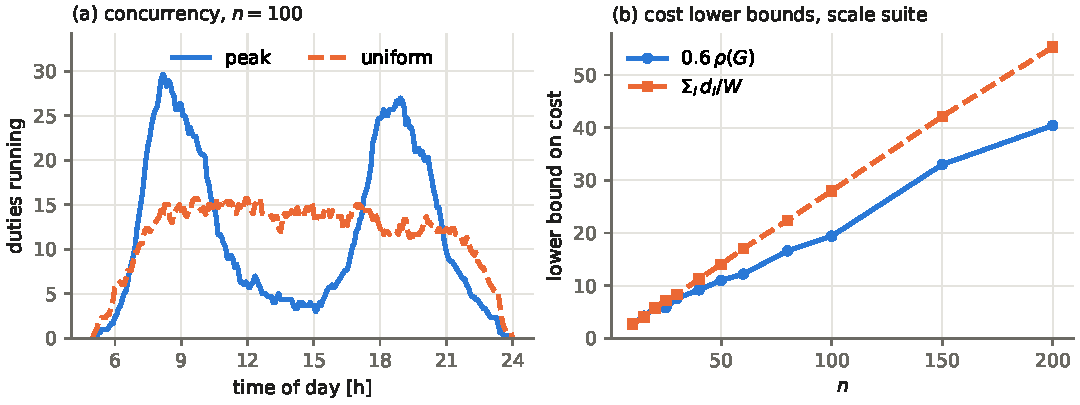
\includegraphics[width=\textwidth]{figures/instances.pdf}
\caption{(a) Number of duties running during the day under the two time
profiles ($n=100$, average of 3 seeds). (b) The two lower bounds on the
optimal cost in the scale group.}
\label{fig:instances}
\end{figure}

\paragraph{Observations.}
\begin{itemize}
  \item \emph{Size.} Density stays near $0.64$ in the scale group, so
    $|\A|$ grows quadratically (from 29 arcs at $n=10$ to about 12\,800 at
    $n=200$). With an employee pool of size $\Theta(n)$, (AF) has
    millions of variables at the top of the range. This is a deliberate
    stress test for the compact models.
  \item \emph{Profile.} The peak profile concentrates the duties in two rush
    hours (Figure~\ref{fig:instances}a): maximum concurrency rises from 10.7
    to 14 at $n=40$ and $\rho(G)$ from 12 to 15.3. Since overlapping duties
    need different employees, peaks drive the number of employees.
  \item \emph{Which bound dominates.} For the default class the two bounds
    are close for small $n$, and the working-time bound dominates from
    $n\approx 25$ (Figure~\ref{fig:instances}b). Short duties reverse this
    ($6.0$ vs.\ $4.7$): the binding factor is then the number of parallel
    duties, not the hours. Long duties make the working-time bound clearly
    dominant ($17.9$ vs.\ $11.2$), and $34\%$ of them can only be covered by
    full-time employees. The duration classes thus move instances between a
    ``covering-type'' and a ``packing-type'' regime.
  \item \emph{Spread limit.} $T$ does not change $G$, but it changes how
    much of $G$ a single employee can use: the effective density goes from
    $0.29$ ($T=600$) to $0.64$ ($T=960$).
  \item \emph{Transfer times.} Their effect on the density is mild ($0.66$
    to $0.61$ from low to high): duties last about two hours, much longer
    than the transfers, so most arcs are decided by the time order alone. To
    control the density directly we therefore rely on \texttt{arc\_drop},
    which lowers it to $0.44$ and $0.26$.
  \item \emph{OR-Library.} These instances are much sparser and the
    working-time bound dominates strongly ($\sum d_i/W\approx 3\times
    0.6\rho$). They extend the size range up to $n=500$ on graphs where only
    (AF) is valid.
\end{itemize}


% ===========================================================================
\section{Initial implementation}
\label{sec:implementation}
% Milestone 2
% ===========================================================================
% ===========================================================================
% Section 3 -- Initial implementation
% ===========================================================================

\subsection{Tools and their choice}

\begin{itemize}
  \item \textbf{Language: Python 3.12.} The bottleneck is the MILP solver,
    not model construction: building the largest model we attempt (4 million
    non-zeros) takes a few seconds. Python lets the generator, the models,
    the validator, the experiment runner and the plots share one code base.
  \item \textbf{Solver: HiGHS 1.16}~\cite{huangfu2018} through its Python
    interface \texttt{highspy}. HiGHS is a state-of-the-art open-source
    MILP solver (branch-and-cut with presolve, cutting planes and primal
    heuristics). It needs no licence, so all results can be reproduced
    exactly by anyone, including the lecturer.
  \item \textbf{Second solver: Gurobi 14} through \texttt{gurobipy}. The same
    code can pass the models to Gurobi, which we use to cross-check the
    results on small instances. A full academic licence was not available
    when the baseline was run: the free licence is limited to 2000 variables
    and constraints, which covers only the verification instances of
    Section~\ref{sec:verification}. A comparison of solvers on the full
    suite is a possible improvement for Section~\ref{sec:improvements}.
\end{itemize}

To guarantee that both solvers receive \emph{exactly} the same model, the
models are not written in a solver-specific modelling language. Each builder
fills a solver-independent container (cost vector, bounds, integrality, and
the constraint matrix stored row-wise in sparse form) that is then passed to
either back-end (\texttt{src/milp.py}).

\subsection{Implementation of the models}

The three compact formulations of Section~\ref{sec:compact} are implemented
in \texttt{src/models/baseline.py}, exactly as written there, with no
preprocessing, symmetry breaking or valid inequalities (these are
improvements, Section~\ref{sec:improvements}):
\begin{itemize}[nosep]
  \item \textbf{(AF)}: one binary per employee and augmented arc;
    constraints~\eqref{af:cover}--\eqref{af:spread}.
  \item \textbf{(CF)}: binaries $y_k$, $x_{ik}$;
    constraints~\eqref{cf:cover}--\eqref{cf:work}, with the conflict set
    $C_\tau$ (time conflicts and pairwise spread conflicts) computed for each
    type.
  \item \textbf{(CF-M)}: as (CF) with only the time conflicts, plus the
    big-$M$ spread constraints~\eqref{cfm} with $M=H$.
\end{itemize}

\paragraph{Employee pool.} The pool sizes are computed as in
Section~\ref{sec:compact} from the cost $\bar z$ of a greedy solution:
$U_{\mathrm F}=\min(n,\lfloor\bar z\rfloor)$ and
$U_{\mathrm H}=\min(n_{\mathrm H},\lfloor\bar z/0.6\rfloor)$, where
$n_{\mathrm H}$ is the number of duties with $d_i\le W/2$. The greedy
(\texttt{src/heuristics/greedy.py}) scans duties by start time and appends
each to the compatible open shift that ended last, opening a new shift when
none fits. It is run once with full-time and once with half-time limits, and
the cheaper result is kept. For (CF) and (CF-M) the greedy only builds
pairwise-compatible shifts. This matters on non-transitive graphs: a pool
sized from a solution that (CF) cannot represent may be too small for (CF),
which is a restriction there (Remark after Proposition~\ref{prop:cf}). We
found this case while testing (Section~\ref{sec:verification}). The greedy
solution is \emph{not} given to the solver as a starting point: the baseline
uses the solver alone.

\paragraph{Size limit.} Models with more than 4 million non-zeros are not
built and are recorded as \emph{too large}. The memory of our machine
(16\,GB, shared by parallel runs) would not allow solving them anyway, and
the limit itself shows how far each formulation scales.

\subsection{Verification}
\label{sec:verification}

\paragraph{Independent validator.} Every solution returned by a solver is
decoded into a list of shifts and checked by \texttt{src/validator.py},
which uses only the instance data and none of the models. It checks that each
duty is covered exactly once, that consecutive duties of a shift are joined
by an arc of $G$, the working-time and total-time limits of the shift's type,
and that the recomputed cost equals the objective reported by the solver.

\paragraph{Hand-crafted instances.} Table~\ref{tab:tests} lists small
instances whose optimal cost we derived by hand; each targets one rule of the
problem. All three models, with both HiGHS and Gurobi, return the expected
optimum, and the validator accepts all their solutions (54 checks). Five
further tests confirm that the validator \emph{rejects} broken solutions: an
HT shift over its working time, a missing duty, a duplicated duty, a wrong
reported cost, and a shift that is not a path in $G$
(\texttt{tests/test\_small.py}).

\begin{table}[ht]
\centering
\small
\caption{Verification instances ($W=480$, $T=720$ unless stated; duty
intervals in minutes; all time-feasible pairs are arcs unless stated).}
\label{tab:tests}
\begin{tabular}{@{}lp{5.0cm}p{5.0cm}r@{}}
\toprule
Name & Duties & What it tests & Optimum \\
\midrule
all\_ht & $[0,100],[110,200]$ & both fit one HT shift & 0.6 \\
overlap & $[0,100],[50,150]$ & overlapping duties & 1.2 \\
work\_binds & $[0,200],[210,400]$ & work $390>W/2$: one FT beats two HT & 1.0 \\
ht\_spread & $[0,60],[600,660]$ & spread $660>T/2$: one FT & 1.0 \\
ft\_spread & $[0,60],[700,760]$ & spread $760>T$: two HT & 1.2 \\
mixed & $[0,200],[210,400],[50,150]$, arc $0\to1$ only & FT $\{0,1\}$ + HT $\{2\}$ & 1.6 \\
long\_duty & $[0,300]$ & $d>W/2$: FT only & 1.0 \\
3-partition & sizes $26,34,40,30,33,37$ back to back, $W=100$ & reduction of
  Proposition~\ref{prop:np} ($m=2$) & 2.0 \\
non\_transitive & $[0,50],[60,110],[120,170]$, arcs $0\to1\to2$ &
  (AF) exact: $0.6$; (CF), (CF-M) restriction: $1.2$ & 0.6 \\
\bottomrule
\end{tabular}
\end{table}

\subsection{Experimental setup}
\label{sec:setup}

All runs use HiGHS with \emph{default} parameters (relative gap tolerance
$10^{-4}$, random seed 0), one thread per run and a time limit of
\textbf{300\,s} for the branch-and-cut. Five runs are executed in parallel on
an Intel Core i5-12500H (12 cores) with 16\,GB of RAM under Windows~11; all
models run under the same conditions. For each run we record
(\texttt{src/run\_experiments.py}, one CSV row per run):
\begin{itemize}[nosep]
  \item model size (variables, constraints, non-zeros) and build time;
  \item the \emph{LP bound}: optimum of the LP relaxation, solved separately
    with a 60\,s limit, which measures the strength of the formulation;
  \item the \emph{root bound}: dual bound at the end of the root node, after
    presolve and HiGHS's cuts, read through a solver callback;
  \item final status, best objective, best bound, gap, number of nodes and
    running time;
  \item the number of FT and HT employees and the validator verdict.
\end{itemize}
Gaps are measured against the lower bound $\max(0.6\rho(G),\sum_i d_i/W)$ of
Section~\ref{sec:inst-stats} and against the greedy upper bound $\bar z$.


% ===========================================================================
\section{Initial computational experiments}
\label{sec:baseline-exp}
% Milestone 2
% ===========================================================================
% ===========================================================================
% Section 4 -- Initial computational experiments and bottleneck analysis
% ===========================================================================

The three formulations were run on the 76 instances of Section~\ref{sec:suite}
(36 of the scale suite, 30 of the factor suite, 10 from the OR-Library) with
the setup of Section~\ref{sec:setup}: 228 runs, about 1.7 hours of wall-clock
time with five runs in parallel. The raw data are in
\texttt{results/raw/baseline.csv}; the tables and the figure of this section
are generated from that file by \texttt{src/analyze\_baseline.py}.

\paragraph{Correctness.} All 189 solutions returned by the solver were
accepted by the validator. Three (CF-M) incumbents at the time limit
(\texttt{scale\_n150\_s2}, \texttt{scale\_n150\_s3}, \texttt{csp100}) were
first flagged because the reported cost was higher than the cost of the
decoded shifts. In these solutions some employees have $y_k=1$ but no duty.
Constraints $x_{ik}\le y_k$ allow this, and it is never optimal, but an
incumbent found early may contain it. The decoded shifts are feasible; the
idle employees add $1.2$--$5.2$ to the cost. The runner now validates the
decoded shifts at their own cost and records the idle cost separately.

\subsection{Results}

\paragraph{Scalability.} Table~\ref{tab:base-scale} and
Figure~\ref{fig:base-scale} show the scale suite. All three models solve
every instance with $n\le 25$. (AF) is the first to fail: it solves all seeds
only up to $n=25$, no instance with $n\ge 40$, and for $n\ge 80$ it does not
even finish the root node, so the solver has no lower bound (gap 100\%). (CF)
solves all seeds up to $n=50$ in a few seconds and stays within 9\% of its
bound at $n=100$. (CF-M) also solves everything up to $n=50$, with a
single exception at $n=40$, but it is 15--30 times slower than (CF) there and
its gap grows faster. Models are \emph{too large} (over 4 million non-zeros)
from $n=150$ for (AF) and (CF), and at $n=200$ for (CF-M), which has half the
constraints of (CF).

\begin{table}[ht]
\centering
\small
\setlength{\tabcolsep}{4.5pt}
\caption{Scale suite: instances solved to optimality (of 3 seeds), mean time
in seconds (300 for unsolved runs) and mean final gap (\%) between incumbent
and solver bound. A gap of 100 means that the root node did not finish, so no
bound was available.}
\label{tab:base-scale}
\begin{tabular}{rrrrrrrrrr}
\toprule
 & \multicolumn{3}{c}{(AF)} & \multicolumn{3}{c}{(CF)} & \multicolumn{3}{c}{(CF-M)} \\
\cmidrule(lr){2-4} \cmidrule(lr){5-7} \cmidrule(lr){8-10}
$n$ & solved & time & gap & solved & time & gap & solved & time & gap \\
\midrule
10 & 3/3 & 0 & 0.0 & 3/3 & 0 & 0.0 & 3/3 & 0 & 0.0 \\
15 & 3/3 & 1 & 0.0 & 3/3 & 0 & 0.0 & 3/3 & 0 & 0.0 \\
20 & 3/3 & 4 & 0.0 & 3/3 & 0 & 0.0 & 3/3 & 1 & 0.0 \\
25 & 3/3 & 18 & 0.0 & 3/3 & 0 & 0.0 & 3/3 & 1 & 0.0 \\
30 & 2/2 & 35 & 0.0 & 3/3 & 4 & 0.0 & 2/2 & 9 & 0.0 \\
40 & \multicolumn{3}{c}{too large} & 1/1 & 1 & 0.0 & 1/1 & 54 & 0.0 \\
\bottomrule
\end{tabular}

\end{table}

\begin{figure}[ht]
\centering
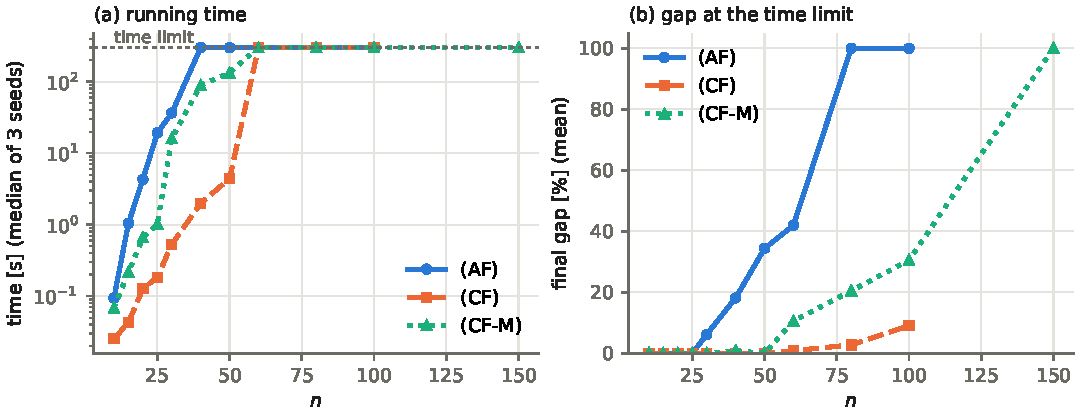
\includegraphics[width=\textwidth]{figures/base_scale}
\caption{Scale suite: (a) running time and (b) final gap as functions of the
number of duties $n$.}
\label{fig:base-scale}
\end{figure}

\paragraph{Formulation strength.} Table~\ref{tab:base-bounds} compares the
bounds with the proven optimum on the 47 transitive instances solved by some
model. The results confirm the theory of Section~\ref{sec:properties}. The LP
relaxation of (AF) is the strongest (19.6\% below the optimum), and the LP of
(CF) and (CF-M) is weak (30.5\%; the two LPs coincide, because spread
constraints are not binding in the LP). The \emph{root} bound, after HiGHS's
presolve and cutting planes, shows a different picture. For (CF) the root gap
drops to 0.8\%, and 40 of its 50 optimal runs need no branching. The
conflict constraints $x_{ik}+x_{jk}\le y_k$ form cliques of pairwise
conflicting duties, and the solver's clique cuts recover what the LP misses.
The big-$M$ spread constraints of (CF-M) do not have this structure: its root
gap stays at 5.5\%, and its solved runs need a median of 1111 nodes. (AF)
improves least at the root (from 19.6\% to 12.2\%). Its LP is slow
(Table~\ref{tab:base-size}), which leaves little time for the cut rounds.

\begin{table}[ht]
\centering
\small
\caption{Bound quality on the transitive instances with a known optimum
$z^*$: mean LP gap $(z^*-z_{\mathrm{LP}})/z^*$ and root gap
$(z^*-z_{\mathrm{root}})/z^*$ (one (AF) run whose root did not finish is
excluded from the root mean), median nodes of the solved runs, runs solved.}
\label{tab:base-bounds}
\begin{tabular}{lrrrrr}
\toprule
Model & instances & LP gap \% & root gap \% & nodes (solved) & solved \\
\midrule
(AF) & 14 & 21.8 & 4.1 & 1 & 14 \\
(CF) & 16 & 34.0 & 0.8 & 1 & 16 \\
(CF-M) & 15 & 34.8 & 1.2 & 1 & 15 \\
\bottomrule
\end{tabular}

\end{table}

\paragraph{Model size and LP time.} Table~\ref{tab:base-size} shows two
typical instances. (AF) has about 15 times more variables than (CF), but
very few rows. Its LP is highly degenerate: the $|\K|$ copies of each arc
are identical, so the simplex method makes many moves that do not change the
objective. At $n=40$ HiGHS needs 23\,s for the LP of (AF), against 0.3\,s
for (CF). At $n=100$ the (AF) LP alone does not finish in 60\,s (14 runs out
of 64). (CF) grows in the other direction: its rows are the conflict
constraints, $O(|\K|\,n^2)$ of them, and this is what makes it too large at
$n=150$.

\begin{table}[ht]
\centering
\small
\caption{Model size and time for the LP relaxation (instances
\texttt{scale\_n040\_s1} and \texttt{scale\_n100\_s1}; pool sizes
$U_{\mathrm F}+U_{\mathrm H}=48$ and $110$).}
\label{tab:base-size}
\begin{tabular}{@{}lrrrrrrrr@{}}
\toprule
& \multicolumn{4}{c}{$n=40$} & \multicolumn{4}{c}{$n=100$} \\
\cmidrule(lr){2-5}\cmidrule(lr){6-9}
Model & vars & rows & non-zeros & LP [s] & vars & rows & non-zeros & LP [s] \\
\midrule
(AF)   & 28\,464 & 2\,104  & 111\,936 & 23.3 & 366\,630 & 11\,430  & 1\,455\,520 & $>60$ \\
(CF)   & 1\,968  & 29\,830 & 91\,194  & 0.3  & 11\,110  & 446\,091 & 1\,348\,753 & 18.0 \\
(CF-M) & 2\,064  & 18\,712 & 54\,000  & 0.3  & 11\,330  & 233\,190 & 688\,050    & 13.1 \\
\bottomrule
\end{tabular}
\end{table}

\paragraph{Primal side.} The solver often finds poor solutions on large
instances. In 14 of the 49 (AF) runs that hit the time limit, the incumbent
is \emph{worse} than the greedy solution used to size the pool. Examples are
$62.8$ against $42.0$ at $n=100$, and $88.8$ against $52.6$ on
\texttt{csp150}. The same happens in 4 of 21 (CF-M) runs, and one (CF-M) run at
$n=100$ ends with no solution at all. (CF) is never worse than its greedy.
The greedy itself is on average 10\% (at most 28\%) above the optimum.

\paragraph{Instance factors.} Table~\ref{tab:base-factor} varies one generator
parameter at a time on $n=40$. (AF) fails on every variant except one sparse
instance (arc\_drop $0.6$), because its size depends on the number of arcs.
For (CF) and (CF-M) a longer total time ($T=960$) and short duties make the
problem easier. A flat demand profile and long duties make (CF) about six
times slower. A plausible reason is that a flat profile has fewer overlapping
duties, so the conflict cliques are smaller. With long duties the working-time
limit binds, and the conflict constraints do not express it. The
strongest effect comes from removing arcs (arc\_drop). The graph is then no
longer transitive and (CF) is a restriction (Remark after
Proposition~\ref{prop:cf}). It becomes slower, and its result can be wrong. On
\texttt{fac\_arc\_drop-0.6\_s3}, (AF) proves an optimum of $16.0$, while (CF)
cannot go below its bound of $16.2$.

\begin{table}[ht]
\centering
\small
\setlength{\tabcolsep}{4.5pt}
\caption{Factor suite ($n=40$, 3 seeds per variant, one parameter changed
from the default): solved, mean time [s], mean final gap [\%].}
\label{tab:base-factor}
\begin{tabular}{lrrrrrrrrr}
\toprule
 & \multicolumn{3}{c}{(AF)} & \multicolumn{3}{c}{(CF)} & \multicolumn{3}{c}{(CF-M)} \\
\cmidrule(lr){2-4} \cmidrule(lr){5-7} \cmidrule(lr){8-10}
Variant & solved & time & gap & solved & time & gap & solved & time & gap \\
\midrule
default & -- & -- & -- & -- & -- & -- & -- & -- & -- \\
profile-uniform & -- & -- & -- & -- & -- & -- & -- & -- & -- \\
durations-short & -- & -- & -- & -- & -- & -- & -- & -- & -- \\
durations-long & -- & -- & -- & -- & -- & -- & -- & -- & -- \\
travel-low & -- & -- & -- & -- & -- & -- & -- & -- & -- \\
travel-high & -- & -- & -- & -- & -- & -- & -- & -- & -- \\
T-960 & -- & -- & -- & -- & -- & -- & -- & -- & -- \\
T-600 & -- & -- & -- & -- & -- & -- & -- & -- & -- \\
arc\_drop-0.3 & -- & -- & -- & -- & -- & -- & -- & -- & -- \\
arc\_drop-0.6 & -- & -- & -- & -- & -- & -- & -- & -- & -- \\
\bottomrule
\end{tabular}

\end{table}

\paragraph{OR-Library.} The OR-Library graphs are not transitive, so only
(AF) is exact on them (Table~\ref{tab:base-orlib}). (AF) solves none of them:
it reaches a gap of 21\% on \texttt{csp50}. From \texttt{csp100} on, its
incumbents are much worse than the greedy, and from \texttt{csp150} it has no
bound. From \texttt{csp250} the model is too large. The restriction (CF) also
pays for non-transitivity before any optimisation. The greedy limited to
pairwise-compatible shifts (greedy$^{\mathrm{pw}}$) is 15--26\% more expensive
than the general one. The (CF) bounds (20.0 and 31.6) bound only the
restriction, not the problem, and on \texttt{csp100} its best solution (38.4)
is worse than the general greedy (33.8). None of the baseline models can
handle realistic OR-Library sizes.

\begin{table}[ht]
\centering
\small
\setlength{\tabcolsep}{4pt}
\caption{OR-Library instances ($W=480$, $T=720$). LB is the combinatorial
lower bound of Section~\ref{sec:inst-stats}; greedy is the general greedy and
greedy$^{\mathrm{pw}}$ the pairwise one used for (CF). The (CF) bound is a
bound of the restriction only. ``none'': the root node did not finish;
``large'': over 4 million non-zeros.}
\label{tab:base-orlib}
\begin{tabular}{rrrrrrrr}
\toprule
 & & & \multicolumn{3}{c}{(AF)} & \multicolumn{2}{c}{(CF) restriction} \\
\cmidrule(lr){4-6}\cmidrule(lr){7-8}
$n$ & LB & greedy & obj & bound & status & obj & bound \\
\midrule
\bottomrule
\end{tabular}

\end{table}

\subsection{Bottleneck analysis}
\label{sec:bottlenecks}

From these results we identify five bottlenecks. Each suggests an improvement
for Section~\ref{sec:improvements}.

\begin{enumerate}[label=\textbf{B\arabic*.}]
  \item \textbf{Size of the compact models.} Both exact formulations index
    every variable by employee, so their size is $|\K|$ times that of a single
    shift: $O(|\K|\,|\A|)$ for (AF) and $O(|\K|\,n^2)$ for (CF). With
    $|\K|=U_{\mathrm F}+U_{\mathrm H}$ up to $2.7\,\bar z$ this limits us to
    $n\le 100$, while the
    OR-Library goes up to $n=500$. \emph{Hypothesis:} a formulation without
    employee index, the set partitioning model (SP) of
    Section~\ref{sec:sp} solved by column generation, removes this
    dependence. Smaller pools, from a better heuristic $\bar z$, would help
    the compact models.
  \item \textbf{Symmetry.} Employees of the same type are interchangeable.
    Any solution has $U_{\mathrm F}!\,U_{\mathrm H}!$ copies, and branching on
    one employee's variable does not move the bound. This explains the many
    nodes of (CF-M) and the degenerate LP of (AF). \emph{Hypothesis:}
    symmetry-breaking constraints ($y_k\ge y_{k+1}$, and assigning
    duty~$i$ only to the first $i$ employees) reduce the nodes and the LP
    time. (SP) has no such symmetry.
  \item \textbf{Weak LP relaxation of (CF).} The 30\% LP gap
    (Proposition~\ref{prop:lp-cf}) is closed only by the solver's clique
    cuts, which are generic and become expensive as the number of rows
    grows; at $n=100$ (CF) does not finish the root node. \emph{Hypothesis:}
    replacing the pairwise time conflicts by \emph{maximal clique}
    constraints $\sum_{i\in Q}x_{ik}\le y_k$, one per maximal set $Q$ of
    pairwise overlapping duties, gives a stronger and much smaller model.
    The time-conflict graph is an interval graph, so it has at most $n$
    maximal cliques and they are found by one sweep over the start times.
  \item \textbf{Poor primal solutions.} The solver often ends with an
    incumbent worse than a simple greedy, or with none. \emph{Hypothesis:}
    passing the greedy as a starting solution (MIP start), and improving it
    with a local search, gives every run a good upper bound from the
    start. It also lets the solver prune more nodes. Removing idle employees
    from the incumbents costs nothing and is always valid.
  \item \textbf{Non-transitive graphs.} (CF) is fast but only a restriction
    when the triangle inequality fails, which is the case on the OR-Library
    and on the arc\_drop instances, and (AF) is exact but too large there.
    \emph{Hypothesis:} (SP), whose columns are paths in $G$, is exact on any
    graph, so it removes this trade-off.
\end{enumerate}

Further, smaller improvements: all costs are multiples of $0.2$, so the
objective scaled by $5$ is integer and any bound $z_{\mathrm{LB}}$ can be
rounded up to $\lceil 5z_{\mathrm{LB}}\rceil/5$. This closes the final gaps
of many time-limit runs at little cost. A second solver (Gurobi, with an
academic licence) would show how much of the difference between the models
is due to HiGHS.


% ===========================================================================
\section{Proposed improvements}
\label{sec:improvements}
% Milestone 3
% ===========================================================================
\TODO{Mathematical and algorithmic description of the improvements.}

% ===========================================================================
\section{Comparative computational evaluation}
\label{sec:comparison}
% Milestone 3
% ===========================================================================
\TODO{Apples-to-apples comparison, performance profiles, conclusions.}

\bibliographystyle{plain}
\bibliography{references}

\end{document}
